\documentclass[a4paper, 12pt, UTF8]{ctexart}
\usepackage{matnoble-doc-cn}
\begin{document}
\title{\bf 拥塞控制算法综述} \author{
\bf \href{https://github.com/baolintian}{田宝林}\quad 
\bf \href{https://github.com/miracleXH}{韩昊轩}} 
\date{}

\maketitle
\tableofcontents
\footnote{\noindent \createtext{2020 年 9 月 21 日} \newline
  \updatetext{\today}}.

\clearpage
%\listoflistings

%\clearpage

\section{背景}
%\zhlipsum[2-3]
\par 尽管TCP协议中的拥塞控制算法已经发展了几十年,但是互联网中的TCP数据包传输效率依然非常的低效。很难有一个拥塞控制算法,能够统一的解决所有性能上的问题,这与它们底层的设计有关:在包的层面硬绑定(Hardwired Mapping)\cite{DongMZAGGS18}了对应的拥塞控制算法。例如,传统的拥塞控制协议是基于数据链路是否丢包进行反应的。一旦产生丢包,那么拥塞控制窗口就会减半。丢包往往可能有两方面的原因\cite{DBLP:conf/imc/SundaresanADC17}:
\begin{itemize}
	\item 数据链路中真的产生了缓冲队列的拥塞,因此需要减小拥塞控制窗口。
	\item 数据链路传输错误,导致数据包丢包。
\end{itemize}

\par 因传输环境和传输介质的不稳定性,第二种情况是有固定的概率产生。但是这种情况下不需要进行拥塞控制窗口减半的操作,因此降低了TCP数据包的传输效率。

\par 随着大规模互联网应用的不断发展,如搜索引擎、视频网站、网络商店,千万级别的数据访问量对数据的访问操作提出了极大的挑战。服务提供商往往有自己的数据中心(Data Center)来处理这些海量的请求,并且合理的分发任务进行高效的处理。在数据传输的过程中,也对服务质量(SLA)提出了挑战。数据中心数据传输和传统的广域网的数据传输有着非常多不同的特点:
\begin{itemize}
	\item 随着大规模集成电路技术的发展,硬件的制造成本越来越低,使得在广域网中的链路设备缓存大小越来越大,链路呈现长肥管道状(long haul network)\cite{BDP}。但是在数据中心中,并不会为了追求低丢包率而设置较大的缓存。相反,为了能够及时的相应的数据请求,往往设置非常小的缓冲区大小。若有较多的数据请求包到来,并且占满了小缓冲区的时候,那么就会直接进行丢包。
	\item 数据中心的时延往往是非常低的,时延的数量级大约是$\mu s$ 级别,因此基于时延的普通拥塞控制协议是很难在数据中心中起来作用的\cite{DBLP:conf/sigcomm/ZakiPCSG15}。
\end{itemize}

\par 因此,将传统的拥塞控制算法应用在数据中心会产生很多的问题,如Vegas\cite{DBLP:journals/jsac/BrakmoP95}, FAST\cite{DBLP:journals/ton/WeiJLH06}拥塞控制算法是基于链路的时延的,数据中心的数据发送时延大约在10微秒左右,因此传统的拥塞控制算法很难准确的测量瓶颈链路的时延,造成数据传输的低效。因此在2010年左右,Microsoft首先推出了DCTCP\cite{DBLP:conf/sigcomm/AlizadehGMPPPSS10}算法,开始了数据中心拥塞控制的分支。

\par 除了传统广域网和数据中心拥塞控制算法的更新和发展,在广域网的拥塞控制算法中细分出了更多的研究门类。目前有下面的几个类别:
\begin{enumerate}
	\item Reno, Cubic等拥塞控制算法先填满整个链路,产生丢包,然后做降速,进行周期调整。
	\item 不使用丢包率作为拥塞调整的信号,而是使用时延信号进行控制。
	\item 特定领域的拥塞控制算法,不再追求一般性。
	\item 基于学习算法的在线/离线拥塞控制协议。
\end{enumerate}
\par 其中传统一类的基于规则控制思想的拥塞控制算法;还有一类使用目前非常热门的机器学习的相关知识,先给定相应的优化模型和优化目标,根据网络中收集到的数据,动态的调整整个拥塞算法的控制参数。

\par 由于网络环境的多变性,如蜂窝网络、无线网络(Adaptive Congestion Control for Unpredictable Cellular Networks)、网页应用、视频传输、有线网络、卫星网络,很难有一个确定统一的算法,能够较为有效的处理所有的网络情况,出现越来越多具体的拥塞控制算法,在特定的领域能够取得较为高效的传输效率。

\par 设计一个新的拥塞控制算法时,需要确定是在应用层做还是在内核层面进行,并且需要和其他的拥塞控制算法进行对比。但是由于测试环境的多样性,太多的研究实践花在复现他人的实验环境和结果,造成了精力的浪费。其次,一个实体的云服务器通过虚拟化的技术来分割成多个虚拟机,从而能够以更细粒度的时间和空间管理有限的计算资源。但是,当租赁用户需要更换拥塞控制协议,他们是没有权限\cite{DBLP:conf/sigcomm/HeRAGFCA16}来进行这样的操作的。有多种研究对新型拥塞控制算法的易用性平台和底层平台\cite{DBLP:conf/usenix/YanMHRWLW18}支持做了很多的努力。希望能够提供一个通用的平台,使用统一的测试环境,从而尽可能减小复现的重复劳作,提高设计和测试的效率。目前主流通用测试平台有CCP\cite{CCP}和Pantheon\cite{Pantheon}。

\par 本Survey主要探索目前主流的拥塞控制算法,给出背后相同的设计思路,给出它们使用的优点和局限性,从而能够更好理解拥塞控制算法根本局限性。

\clearpage

\section{各类网络的特点}
\par 由于网络系统环境的多变性,我们首先需要了解一些网络场景中的特点,从而能够帮助我们更好的理解需要解决的场景问题,同时能够更好的理解每种特定网络的拥塞控制协议背后设计的思想,最后能够方便我们对相应的网络进行模拟(Simulation)和仿真(Emulation)。

\subsection{广域网}
\begin{itemize}
	\item 在建立网络基础设备的初期,往往硬件的缓冲区大小是非常小的。随着摩尔定律的发展,硬件的容量已经不再是问题,因此目前的网络链路的特点为长肥管道状(Long Haul Network)。\cite{BDP}
	\item 数据流速度变化非常的大,网络变化大。例如在生活中,有时候在视频网站上看视频可能会无常的出现视频卡顿的现象。
\end{itemize}

\subsection{数据中心}

\begin{itemize}
	\item Incast: 大量的小数据请求同时从机架(Racks)发往中心处理点(Aggregator),然后填满了缓冲区,使得丢包,发出重传信号,超时重传时间(Retransmission Timeout)在客户端一般是100ms左右,而数据中心的时延一般小于1ms,这样就导致数据中心会等待客户端的重传。降低了90\%Throughput\cite{DBLP:conf/sigcomm/AlizadehGMPPPSS10}。
	\item 带宽为1-40Gbps,时延非常的低,微秒级别。
\end{itemize}

\subsection{移动网络}

\begin{itemize}
	\item 短时间内网速变化非常大
	\item 自身导致的排队时延
	\item 与拥塞控制无关的丢包
\end{itemize}

\subsection{卫星网络}
\begin{itemize}
	\item 较高的随机丢包率
	\item 高时延
\end{itemize}

\clearpage

\section{优化目标}
\par 衡量网络好坏往往有非常多的指标,不同的网络系统往往追求的指标是不相同的。如股票交易系统、实时网络游戏的网络对时延有着非常高的要求;网络视频、网络语音往往对网络的丢包率有较高的要求。这些系统背后往往会有某个具体的拥塞控制协议来控制管理的。论文《An Experimental Study of the Learnability of Congestion Control》\cite{DBLP:conf/sigcomm/SivaramanWTB14}描述了一个在上帝视角(Omniscient)的全能型的拥塞控制算法,在所有的性能方面都是最优的。下面将列出几个通用的测量指标,方便通过这些指标的变化来评价具体拥塞控制算法的好坏,同时也能够更好的知道网络中的优化目标。


\subsection{高带宽}
\par 一些长连接(Long Term Connection)追求高吞吐,是主要的优化的目标的应用场景。一些短连接对低时延有较高的要求。
\subsection{低时延}
\par 在广域网中,由于现在网络互联设备不断的更新,内存越来越廉价。因此,广域网中呈现长肥管道的现象越来约明显。因此时延很难控制。

\par 在数据中心内部,一般的做法就是减小缓冲区的大小,从而能够减小排队时延。

\subsection{丢包率}
\par 比较传统的拥塞控制算法是基于丢包这个指标进行拥塞控制的,使得在没有发生丢包动作的时候,算法会拼命的往链路中发送数据包,来填满整个链路,因此这个策略往往丢包率是比较低的。在进行控制的过程中,丢包率也是一个非常重要的一项指标。

\subsection{竞争性}

\par 不同种类TCP数据流\cite{DBLP:conf/imc/WareMSS19}公平性是非常重要的,虽然每种拥塞控制算法优化指标有不同,但是在竞争性问题上还是必须达成一致的。由于互联网底层的发展还是非常的缓慢的,其中保存着很多约定俗成的规则。若轻易的破环数据链路公平竞争的性质,那么会产生恶意竞争的情态,造成互联网的混乱。
\par 设有n个数据流,每个数据流的流速为$f_i$,评估指标为Jain index:
$$
index(f_1, f_2,…,f_n)=\frac{(\sum_{i=1}^{n}f_i)^2}{n*\sum_{i=1}^nf_i^2}
$$
该数值的取值范围为0-1,越接近1表示越公平。

\subsubsection{竞争性问题的探讨}
\par 关于网络链路公平竞争是一个非常重要的问题,因为网络设备的更新往往是非常慢的,中间链路存在着很多的较陈旧拥塞控制算法。若此刻新的拥塞控制算法加入网络,导致数据链路中的旧的拥塞控制算法无法公平的占有应有的带宽资源。若对这种情况放任不管,势必会导致拥塞控制算法的恶性发展,甚至会导致整个网络大面积拥塞而最终谁都得不到好处。

\par 正是对公平性的考虑,BBR拥塞控制算法对链路带宽资源的抢占较为的激进,有研究表示\cite{DBLP:conf/sigcomm/SivaramanWTB14},在16条Cubic控制的网络终端和一条BBR控制的网络终端,它们共享一个带宽链路时,一条BBR控制的链路会占用50\%的带宽资源。随后的迭代版本v2\cite{bbrv2}中,BBR取消了较为激进的拥塞控制策略,一定程度上缓解了公平性的问题。

\par 然而,这样的共识却不一定是强制的。明面上,所有经过大规模部署的拥塞控制算法必须遵循这样的准则。但是存在着非常多的"改进版"的拥塞控制算法,它们往往会疯狂的抢占带宽资源,而不会在意整个链路的公平性,如BBR魔改版,锐速等等\cite{linux-netspeed}广为流传的拥塞控制协议应用。

\clearpage

\section{主要拥塞控制算法}
通过调研,发现拥塞控制算法使用的信号各不相同。及时是使用了相同的信号量,采集的方式,处理的方式也千差万别,这就造成了拥塞控制算法的多样性。主要的拥塞信号包括时延和丢包率\cite{congestionControlCategory}。下面我们将通过具体的算法,看看这些信号是如何被利用的。

\subsection{广域网一般拥塞控制算法}

\subsubsection{Reno}
\begin{figure}[H]
	\centering 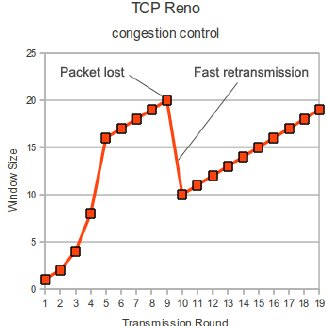
\includegraphics[width=0.6\textwidth]{reno.jpg}
	\\ \hspace*{\fill} \\
	\caption{\em reno控制拥塞控制窗口变化}
	\label{fig:reno algorithm}
\end{figure}
\par 结合图\ref{fig:reno algorithm}, 可以将整个拥塞控制的流程分成四个部分,主要是下面的步骤:
\begin{enumerate}
	\item 慢启动:当不发生丢包的时候,每一个RTT后cwnd翻倍
	\item 当目前拥塞控制窗口的大小超过原来预设的定值的时候,开始每一个RTT,cwnd+1,并且更新阈值的大小
	\item 快重传:当产生丢包后,拥塞控制窗口的大小立刻减半。
	\item 若没有丢包,每一个RTT后拥塞控制窗口的大小+1
\end{enumerate}


\subsubsection{Cubic}
\par Cubic算法\cite{10.1145/1400097.1400105}是对二分法的一个优化,目标是能够拟合出一个合适的三次曲线如图\ref{fig:cubics algorithm}所示,使得在探测拥塞控制窗口的大小的时候能够减小丢包的数量,从而能够减小对中间链路缓冲区的冲击,同时该方法在离阈值较远的时候,也能很快的收敛到阈值的附近。相当于是利用一些已知的信息,进行曲线的拟合与逼近。

\begin{figure}[H]
	\centering 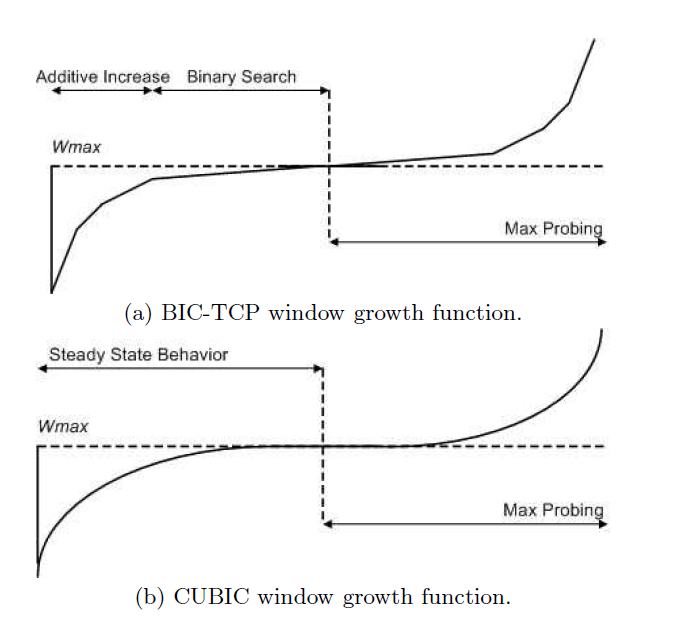
\includegraphics[width=0.6\textwidth]{cubic.png}
	\\ \hspace*{\fill} \\
	\caption{\em cubic拥塞控制窗口增长曲线}
	\label{fig:cubics algorithm}
\end{figure}

\subsubsection{PCC}
\par PCC\cite{DongMZAGGS18}是一类学习类算法,其选择优化的目标:
\begin{enumerate}
	\item Throughput: 越高越好
	\item Loss: 没有因拥塞控制而产生丢包
	\item Latency: 越低越好
\end{enumerate}
\par 其背后的思想很简单:就是以观察到的性能来评判速率变化的方向。在整个控制算法流程中要求输入一组参数,能够实时的调整整个拥塞控制算法协议栈中的各种参数,能够达到最大的利用率。
$$
u(x_i, \frac{d(RTT_i)}{dT}, L_i) = x_i^t-bx_i\frac{d(RTT_i)}{dT}-cx_iL_i
$$
\par 其中b, c都是需要预先确认的常数。在本篇论文中,b=900, c = 11.35。其中c阈值越大,那么能够容忍的丢包率越大。b值的设置与多流的竞争有关系,文中目标1000个用户在1000Mbps的链路中竞争带宽的时候不会产生较大的抖动(Inflation)。

\subsubsection{BBR}
\par BBR\cite{DBLP:journals/queue/CardwellCGYJ16}拥塞控制算法如图\ref{fig:BBR process}所示。一个循环的周期为8RTT,其中包含探测期(ProbeBW),排空期(Drain),稳定期(Steady State), 前两个状态分别会持续1RTT,后面的稳定期会持续6RTT。探测期会主动的多发包,排空期会主动的减少发包的数量,在这个时间段内会探测整个链路的链路的带宽。大约每10s,网络链路就会对最小RTT进行更新。

\begin{figure}[H]
	\centering 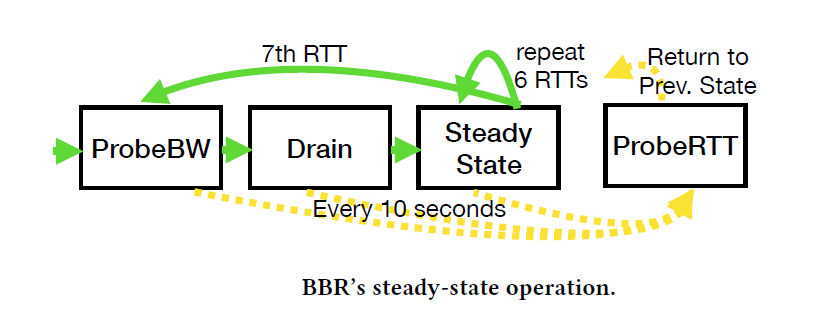
\includegraphics[width=0.6\textwidth]{bbr1.png}
	\\ \hspace*{\fill} \\
	\caption{\em BBR算法控制流程}
	\label{fig:BBR process}
\end{figure}

\par BBR算法不依照丢包率为指标进行探测。如图\ref{fig:BBR algorithm}所示,CUBIC一类以丢包为拥塞控制信号进行控制的算法,实际上在黄实线和红虚线交点处进行不断的探测,并且在周围进行动态的工作。

\begin{figure}[ht]
	\centering 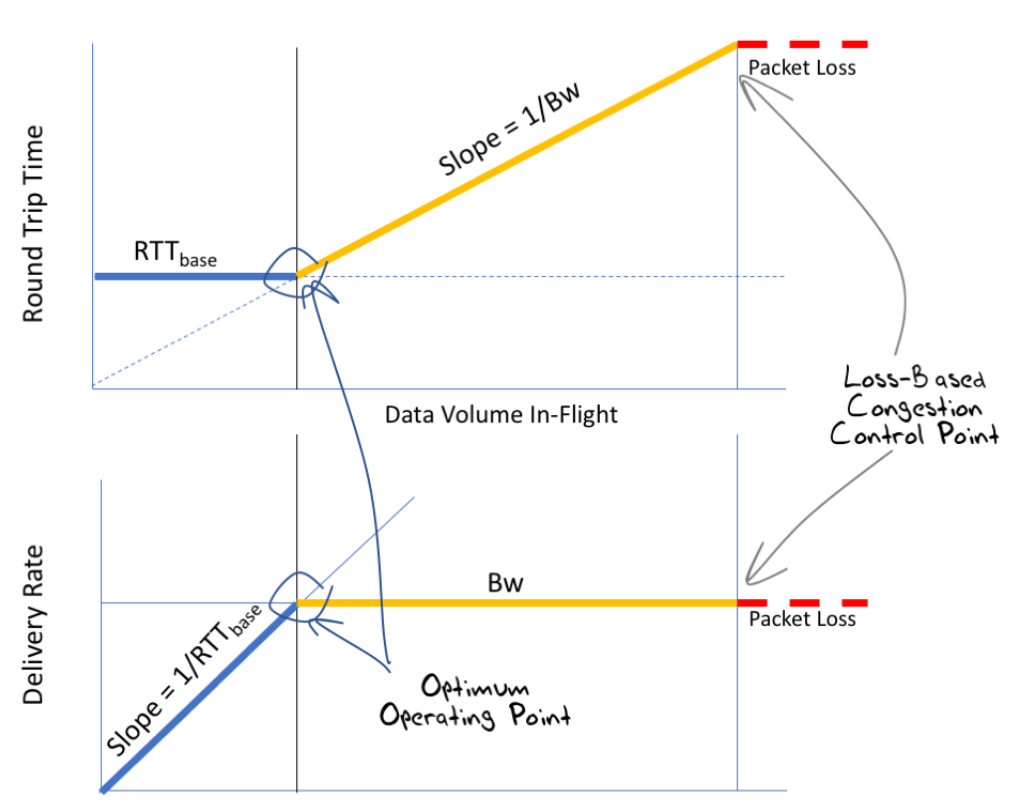
\includegraphics[width=0.6\textwidth]{bbr.png}
	\\ \hspace*{\fill} \\
	\caption{\em BBR、Cubic探测点的区别}
	\label{fig:BBR algorithm}
\end{figure}
\par 但是这样的问题是会主动的填满链路中的缓冲区,从而造成链路的拥塞,甚至会产生Bufferbloat的问题。BBR算法主要探测的点为蓝实线和黄实线相交的地方。这样不会主动的去抢占链路中的缓冲区的大小。

\par 简单来讲,就是通过动态的测量瓶颈链路(Bottleneck Network)中的瓶颈带宽($BBR.BtlBw$)和检测窗口内的瓶颈链路的传输时延(BBR.RTProp),从而两者的乘积产生BDP(Bandwidth Delay Product)。从而去影响整个BBR Engine中的三个参数: $pacing rate$,$send quantum$和$cwnd$。


%\subsubsection{QUIC}
%优点:
%1. 弱网络的时候能够提升 20\% 以上的访问速度\\
%2. 频繁切换 4G 和 WIFI 网络的情况下,不会断线,不需要重连,用户无任何感知。\\
%3. 接入的用户网络环境也千差万别,结合大数据及人工智能处理,我们能为各个用户提供不同的但又更加精准更加有效的拥塞控制。比如 BBR 适合,Cubic 适合\\
%4. \\

\subsubsection{Copa}

\par 学习类的算法在多变的网络环境下性能比较的好,但是不具有解释性\cite{DongMZAGGS18},能够合理的解释目标函数中的常数的含义往往是非常困难的。

%reasoning about fundamental tradeoffs in parameter settings is difficult

\par Copa\cite{DBLP:conf/nsdi/ArunB18}的目标就是在提高可用性的同时,具备很好的解释性。

\par 目标:高速率,低时延,公平竞争。看似前两者是相矛盾的,实际上是Copa不会主动的抢占链路中的Buffer的大小。但是若链路中有了新的数据流的加入,那么Copa会开启竞争模式(开启该模式的指标为RTT的抖动大小),从而抛弃低时延的目标,保证传输的速率。

\par 一开始,我们定义一个目标函数:
$$
U = \log\lambda-\delta \log d
$$
\par 其中 $\lambda$是平均流量,$\delta$是一个权重系数,$d$表示包的时延。

\par 若要使得U最大,那么平均流量$\lambda$:
$$
\lambda_t = \frac{1}{\delta d_q}
$$
$$
d_q = RTT_{standing}-RTT_{min}
$$
$RTT_{standing}$表示在$ \tau = \frac{sRTT}{2}$采样窗口求得,$RTT_{min}$是在较长一段时间内测得的,一般是10s左右。

\par 每收到一个ACK,就进行下面的更新:\\
\begin{itemize}
	\item 若瞬时速率$\lambda = \frac{cwnd}{RTT_{standing}}\le \lambda_{t}$,那么$cwnd = cwnd+\frac{v}{\delta cwnd}$
	\item 否则$cwnd = cwnd - \frac{v}{\delta cwnd}$\\
\end{itemize}

\par 其中$v$是一个参数,相当于是包增减的变化快慢的常数,初始化设置为1。可以得到下面直观的理解:每过一个$RTT$,$cwnd$大约增加$\frac{v}{\delta}$。

\par 若要使得拥塞控制窗口进行快速的收敛,那么如果前一个状态为$cwnd$增加,现状态$cwnd$也是增加的,那么$v=2*v$,并且进行拥塞窗口的更新。图\ref{fig:copa algorithm}是整个拥塞控制算法的流程,以一个数据流为例,当多流时情况类似。
\begin{figure}[H]
	\centering 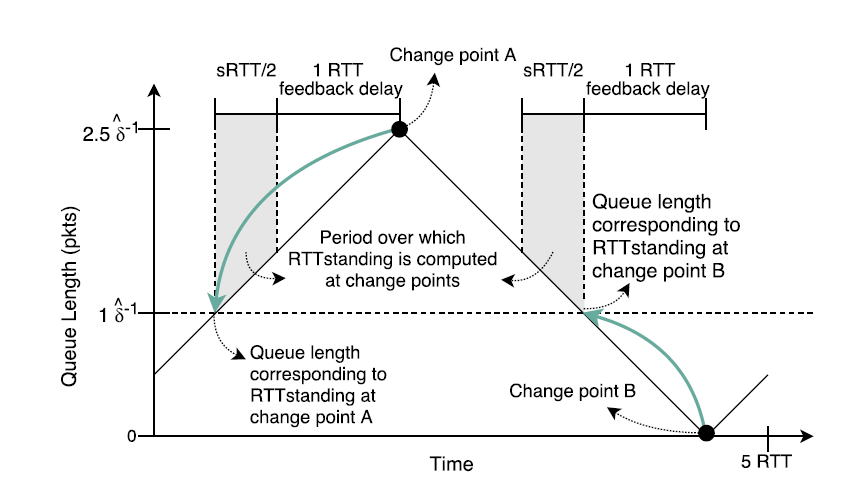
\includegraphics[width=0.8\textwidth]{copa.png}
	\\ \hspace*{\fill} \\
	\caption{\em copa变化情况}
	\label{fig:copa algorithm}
\end{figure}

\par Copa是一个周期性进行探测的过程,每一个周期为5RTT如图\ref{fig:copa algorithm}所示。

\par 为什么是5RTT而不是2RTT呢?首先根据纳什均衡的原理,作者给出了一套理论,当队列中排队的数据包达到$\delta^{-1}$时达到竞争均衡。此后进行$RTT_{standing}$的探测,大约持续的时间为$\frac{RTT}{2}$的时间,因为数据包传输需要1RTT,因此只有达到Change Point A时得到$RTT_{standing}$。反过来的状态类似,直到排空队列中的数据包为止。然后进行周期性的测量与控制。

\subsection{数据中心拥塞控制算法}

\subsubsection{DCTCP}

\par DCTCP\cite{DBLP:conf/sigcomm/AlizadehGMPPPSS10}需要在发送端、接收端、交换机中同时进行布置。交换机中设置有常数$K$,一旦队列中数据包的数量超过这个常数,那么交换机就会在数据包中设置CE(Congestion Expericed) Checkpoint的标志位。

\par 当接收端收到标记的数据包时,本应该立刻发送带有ECN-echo标记位的ACK,但是由于ACK Compression的应用,于是又使用了一个如图\ref{fig:dctcp sm algorithm}所示的2 State Machine状态机,从而能够维持Delayed ACK的性质。

\begin{figure}[H]
	\centering 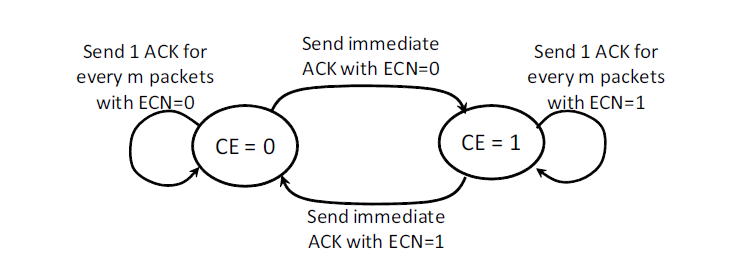
\includegraphics[width=0.8\textwidth]{dctcp.png}
	\\ \hspace*{\fill} \\
	\caption{\em 接收端的状态机}
	\label{fig:dctcp sm algorithm}
\end{figure}

\par 发送端开始统计有多少的数据包被标有CE Checkpoint,并且维护下面的式子:
$$
\alpha = (1-g)\alpha+gF
$$
\par $F$表示的是在一个时间窗口内收集到的标记有CE Checkpoint的数量,$g$是一个权重的系数,$\alpha$表示队列中遇到拥塞的概率的大小,$\alpha \in [0, 1]$。通过更新$\alpha$,从而更进一步的维护$cwnd = cwnd*(1-\frac{\alpha}{2})$

\par 当$\alpha$很小的时候,cwnd保持一个叫小的变化;当$\alpha$接近1的时候,cwnd以指数级别的速率开始减小。

\subsubsection{TIMELY}
\par 随着硬件路由器的发展,RTT精度已经达到了毫秒级别的精度。同时为了避免ACK Compression等问题,TIMELY\cite{DBLP:conf/sigcomm/MittalLDBWGVWWZ15}使用的指标并不是单一的RTT指标,而是RTT梯度。

\clearpage

\section{拥塞控制算法参数的其他应用}
\par 拥塞控制算法利用数据包携带的若干信息,对复杂多变的网路链路进行主动探测。因此,目前有一些研究结合拥塞控制算法,利用其中的一些参数对网络进行评估,从而能够给产品用户最佳的网络产品使用体验。

\subsection{视频画质选择}
\par 在传输视频前,视频网站往往会发送少量的数据包进行探测,试图找到最佳的画质\cite{DBLP:conf/nsdi/YanAZFHZLW20},使得用户在享受视频服务的同时,不会出现卡顿的情况,提高了用户的体验。具体的原理时通过少量的数据包的传输,可以准确知道网络速率。从而能够花很小的开销,动态的调整传输视频的画质。

\subsection{网络测速}
\par 传统的网络测速是使用UDP数据包充满(Saturate)整个数据链路,不管丢包的数量,从单位时间内发送的数据包的数量来推测整个链路的传输速率。然而这种方法首先没有考虑链路中是否拥塞的情况,即使数据包充满了整个链路,但是测量的结果可能依旧会偏低,这是网络提供商不希望用户所看到的。
\par 若使用一些带有速率探测的拥塞控制协议,如BBR,首先可以使用拥塞控制算法探测链路是否拥塞,如果拥塞的话可能提早的告诉用户,能够提供更准确的测速不准的原因\cite{DBLP:conf/imc/SundaresanDFLD17}。其次,基于拥塞控制的网络链路测速不用充满整个链路,从而能够减少数据包的发送,较好的节省了数据流量。


\clearpage 

\section{Testbed设计}
\par 适用于拥塞控制算法的Testbed曾经全是依靠开发者自行针对目标网络系统开发的测试应用,近年来出现了通用的Testbed平台。
\subsection{Pantheon}
\par Pantheon是一个用于研究和评估端到端的网络系统的分布式协作平台,特别针对拥塞控制方案、传输协议以及网络仿真器。旨在解决大型网络系统的拥塞控制测试需要开发人员单独开发拥塞控制算法和传输协议的测试平台的问题。
\par Pantheon生成网络仿真器,网络仿真器经过校准后匹配到真实的网络路径,对仿真器分级的指标是描述一组算法的端到端性能,例如吞吐量、延迟和丢包率,通过在仿真网络上运行算法,根据端到端的性能信息与真实网络中的相同性能统计信息的路径进行匹配。
\par Pantheon被用于了Vivace和Copa算法等的测试工作。一系列的应用也证实了Pantheon既可以将完整的算法部署并测试,也可以进行自动部署和原型测试。通过测量多种传输协议和拥堵控制算法,Pantheon为研究和改进它们的性能提供了一个训练场所。此外,通过生成匹配现实路径的校准仿真器,Pantheon使研究人员能够重复和准确地测量协议及算法\cite{DBLP:conf/usenix/YanMHRWLW18}。

\subsection{CCP}
\par CCP是一个在数据路径之外进行复杂的拥塞控制算法的测试与评估的系统。数据路径指代数据包在网络上被发送时经由的路由器和交换机的顺序。不同于以往的将拥塞控制算法编译到内核中,CCP在应用层进行拥塞控制,提出了利用数据包的数据路径以及在数据路径上传输时的拥塞信号(包括RTT,接收,丢失等)的信息,在一个数据路径之外的模块上进行拥塞控制,使数据路径按照指定的拥塞控制策略传输数据,进行拥塞控制算法的测试。
\par CCP使得测试人员只需要编译一次拥塞控制算法,即可在所有支持指定接口的数据路径上运行。
同时CCP与ACK时钟解耦,用户可以不受包确认的时间限制,从而开发更加灵活的拥塞控制算法\cite{DBLP:conf/sigcomm/NarayanCRGNMAB18}。
\clearpage

\section{个人观点}
\begin{enumerate}
	\item 随着互联网的发展,普适的拥塞控制算法越来越难以满足特定领域的网络指标的需求,随着目标和需求的不断的改变,针对某个特定领域的拥塞控制协议将会越来越多。
	\item 尽管最近十年来,机器学习不断的发展深入到了各个领域,但是在网络的拥塞控制领域,性能指标可能有时候还不如一些传统的拥塞控制算法。其原因如机器学习的较难的解释性,很难解决网络链路中纷繁复杂的网络状况,不能成为主流的拥塞控制算法。
	\item 利用拥塞控制算法中对链路精准估计的参数,也能提高其他应用服务质量。可以说明拥塞控制是系统层较为基础,非常重要的一个控制模块。
\end{enumerate}


\clearpage

\section{Misc}

\begin{enumerate}
	\item 基于一个目标函函数的"学习"类算法,他们设计的这个函数往往是非常巧妙的。这涉及到另外一个关于设计目标函数的一般准则:当有多个需要考虑的目标量时,怎么将不同量纲的参数统一到一个式子里面。Copa使用的方法是使常系数也带有单位,这显然是一个不太好的应用;PCC使用的方法是统一量纲,但是依旧有一个问题,就是每个式子带有的常参数往往很难解释清楚,并且这些常数的量级差距还是很大的,需要有一个自动调节的算法,来达到算法原来设计的目的。
	\item Congestion window在发送端,TCP Sliding Window在接收端,不要将两者混淆了,并且本文主要的研究对象为Congestion Window。
\end{enumerate}

\clearpage


\bibliographystyle{plain}%设置参考文献的类型 (bibliography style). 标准的为 plain
\bibliography{enhance-ref}%告诉LaTeX生成参考文献列表  enhance-ref.bib 是同目录下的参考文献管理文件

\end{document}
